\section{Simulation Analysis}
\label{sec:simulation}

\subsection{Frequency Analysis}

The frequency analysis was done in order to obtain the gain of the circuit as a function of the frequency. \par
The following plot shows the function we obtained for $V_{out}$, in dB, and it is also presented a plot of the phase function.

\begin{figure}[h] \centering
\includegraphics[width=0.5\linewidth]{vo1f.pdf}
\caption{vOUT (dB)}
\label{fig:vOUT}
\end{figure}
\FloatBarrier

\begin{figure}[h] \centering
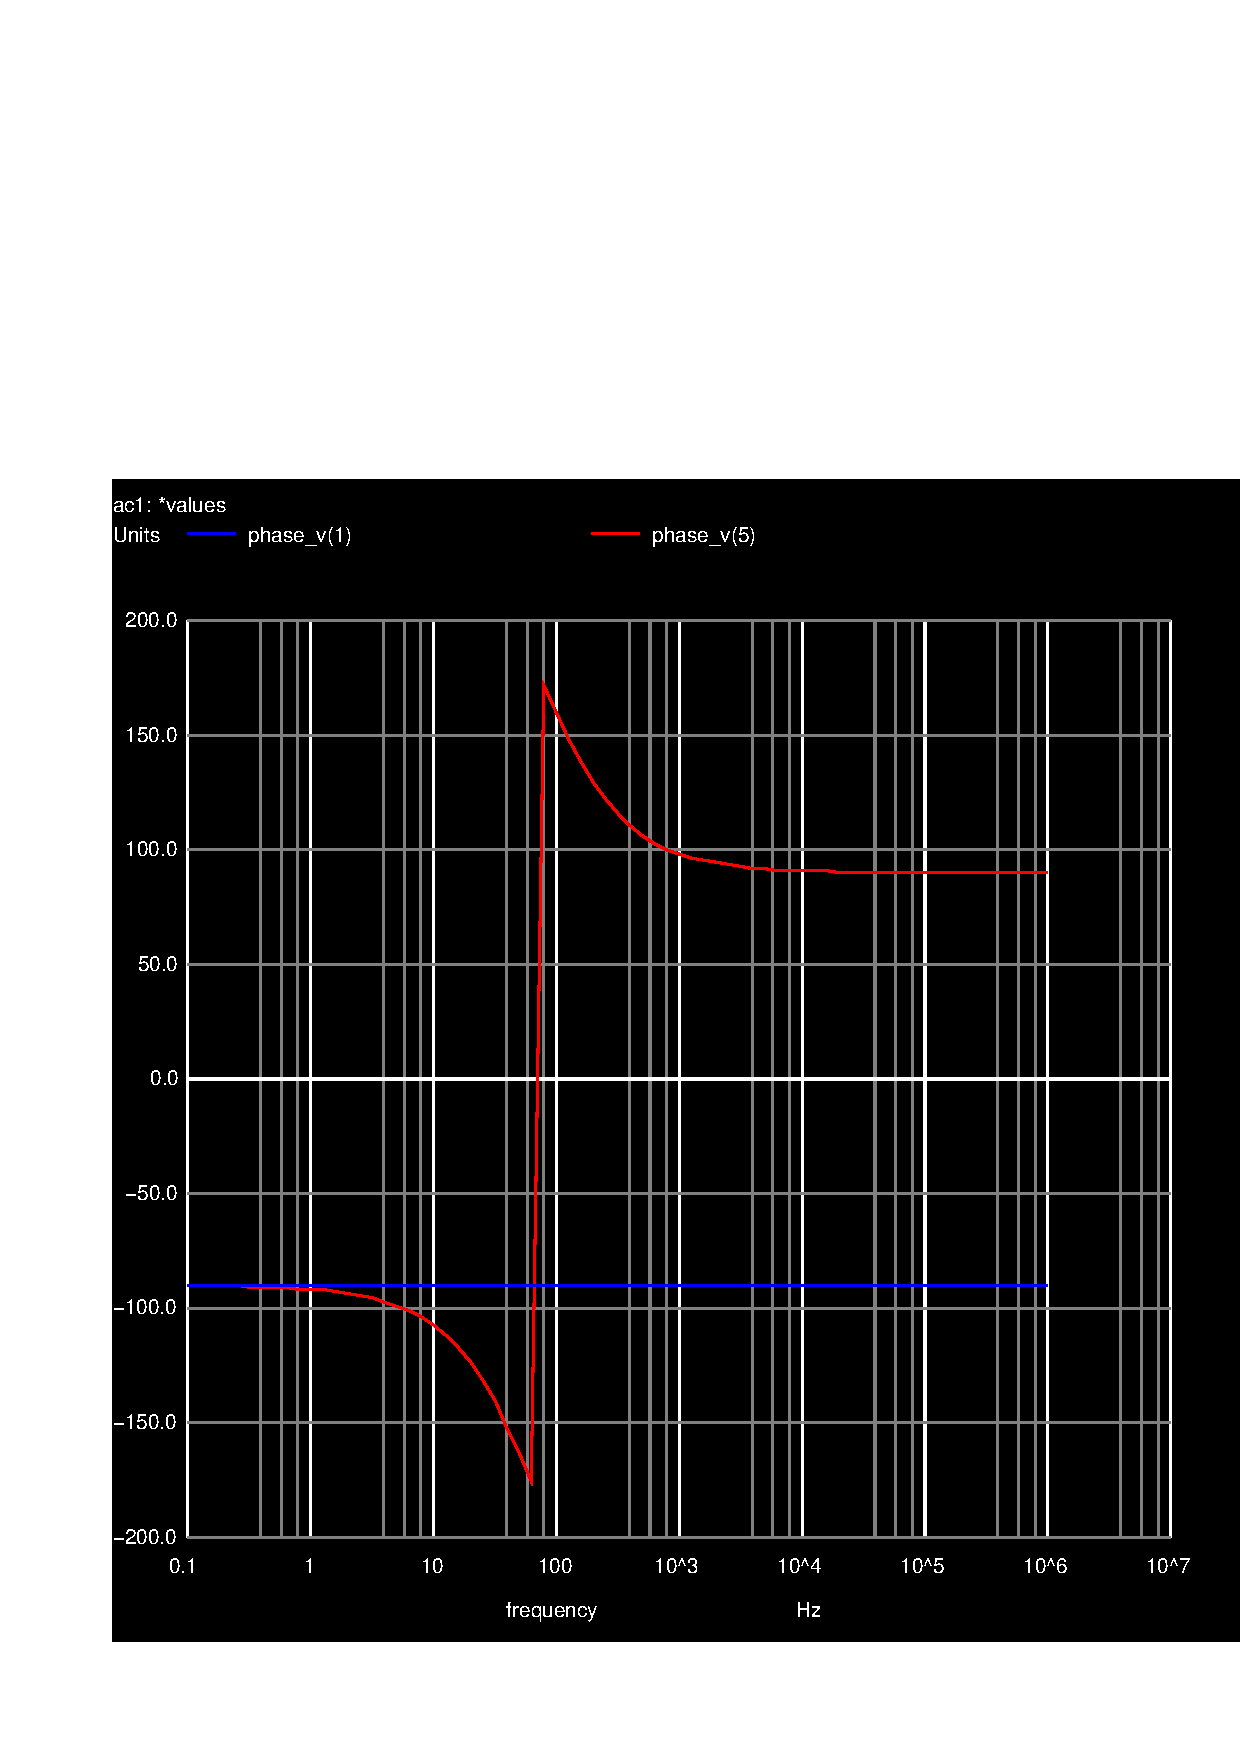
\includegraphics[width=0.5\linewidth]{phase.pdf}
\caption{phase (degrees)}
\label{fig:phase}
\end{figure}
\FloatBarrier

From this analysis, we can also obtain the values for the output voltage gain in the passband, the central frequency, and the input and output impedances at this stage.

\begin{table}[h]
  \centering
  \begin{tabular}{|l|r|}
    \hline    
    {\bf Name} & {\bf Value [dB]} \\ \hline
    z_in1 & 5.638527e+02,-8.44302e+01\\ \hline
gain & -7.85216e+01,-1.54185e+00\\ \hline
lco & 8.880418e+03\\ \hline
uco & 1.603742e+06\\ \hline
bandwith & 1.594862e+06\\ \hline
cost & 1.013002e+05\\ \hline
merit & -1.39209e-01,-2.73352e-03\\ \hline

  \end{tabular}
  \caption{Gain, output and input impedance}
  \label{tab:data1sim_sim}
\end{table}
\FloatBarrier

We can also obtain the values for the upper, lower cut off and central frequencies.

 \begin{table}[h]
  \centering
  \begin{tabular}{|l|r|}
    \hline    
    {\bf Name} & {\bf Value [Hz]} \\ \hline
    uco & 3.106930e+06\\ \hline
lco & 7.923603e+00\\ \hline
bandwith & 3.106922e+06\\ \hline

  \end{tabular}
  \caption{Frequencies}
  \label{tab:data2sim_sim}
\end{table}
\FloatBarrier

\subsection{Merit Figure}
In this section, we present the costs of the components and the total cost of the circuit, as well as the merit figure.

 \begin{table}[h]
  \centering
  \begin{tabular}{|l|r|}
    \hline    
    {\bf Name} & {\bf Value [Hz] [Mu]} \\ \hline
    cost & 8.116008e+03\\ \hline
merit & 2.707518e+03\\ \hline

  \end{tabular}
  \caption{Merit figure}
  \label{tab:data3sim_sim}
\end{table}
\FloatBarrier

\section{In-person simulation}
\label{sec:irl}

Due to the lack of time during the laboratory class, we couldn't build the entire circuit. However, we were able to make some measurements of interest. \par
The $V_{cc}$ tension read in the multimeter was of value $10.097 V$ and the $V_{cc}^-$ tension was of magnitude $-10.030 V$. \par
The input amplitude of the signal was read and measured with the oscilloscope which registered $0.221 V$ and the output amplitude registered $2.450 V$. This translates in a gain of about $11.086V$, which is close to the pretended gain. \par
Due to the pandemic, we couldn't attend laboratory classes during the semester, so this last laboratory assignment showed us that it is not easy to build circuits and that values can vary with lots of outside factors. The programming skills aquired are surely useful, but some hands-on experience in the future will be a good improvement in our skill set.  


\begin{figure}[h]
\centering
  \centering
  \includegraphics[scale=0.1]{in-person.jpg}
  \caption{instruments}
  \label{fig:1}
\end{figure}

